% Options for packages loaded elsewhere
% Options for packages loaded elsewhere
\PassOptionsToPackage{unicode}{hyperref}
\PassOptionsToPackage{hyphens}{url}
\PassOptionsToPackage{dvipsnames,svgnames,x11names}{xcolor}
%
\documentclass[
  letterpaper,
  DIV=11,
  numbers=noendperiod]{scrartcl}
\usepackage{xcolor}
\usepackage{amsmath,amssymb}
\setcounter{secnumdepth}{5}
\usepackage{iftex}
\ifPDFTeX
  \usepackage[T1]{fontenc}
  \usepackage[utf8]{inputenc}
  \usepackage{textcomp} % provide euro and other symbols
\else % if luatex or xetex
  \usepackage{unicode-math} % this also loads fontspec
  \defaultfontfeatures{Scale=MatchLowercase}
  \defaultfontfeatures[\rmfamily]{Ligatures=TeX,Scale=1}
\fi
\usepackage{lmodern}
\ifPDFTeX\else
  % xetex/luatex font selection
\fi
% Use upquote if available, for straight quotes in verbatim environments
\IfFileExists{upquote.sty}{\usepackage{upquote}}{}
\IfFileExists{microtype.sty}{% use microtype if available
  \usepackage[]{microtype}
  \UseMicrotypeSet[protrusion]{basicmath} % disable protrusion for tt fonts
}{}
\makeatletter
\@ifundefined{KOMAClassName}{% if non-KOMA class
  \IfFileExists{parskip.sty}{%
    \usepackage{parskip}
  }{% else
    \setlength{\parindent}{0pt}
    \setlength{\parskip}{6pt plus 2pt minus 1pt}}
}{% if KOMA class
  \KOMAoptions{parskip=half}}
\makeatother
% Make \paragraph and \subparagraph free-standing
\makeatletter
\ifx\paragraph\undefined\else
  \let\oldparagraph\paragraph
  \renewcommand{\paragraph}{
    \@ifstar
      \xxxParagraphStar
      \xxxParagraphNoStar
  }
  \newcommand{\xxxParagraphStar}[1]{\oldparagraph*{#1}\mbox{}}
  \newcommand{\xxxParagraphNoStar}[1]{\oldparagraph{#1}\mbox{}}
\fi
\ifx\subparagraph\undefined\else
  \let\oldsubparagraph\subparagraph
  \renewcommand{\subparagraph}{
    \@ifstar
      \xxxSubParagraphStar
      \xxxSubParagraphNoStar
  }
  \newcommand{\xxxSubParagraphStar}[1]{\oldsubparagraph*{#1}\mbox{}}
  \newcommand{\xxxSubParagraphNoStar}[1]{\oldsubparagraph{#1}\mbox{}}
\fi
\makeatother


\usepackage{longtable,booktabs,array}
\usepackage{calc} % for calculating minipage widths
% Correct order of tables after \paragraph or \subparagraph
\usepackage{etoolbox}
\makeatletter
\patchcmd\longtable{\par}{\if@noskipsec\mbox{}\fi\par}{}{}
\makeatother
% Allow footnotes in longtable head/foot
\IfFileExists{footnotehyper.sty}{\usepackage{footnotehyper}}{\usepackage{footnote}}
\makesavenoteenv{longtable}
\usepackage{graphicx}
\makeatletter
\newsavebox\pandoc@box
\newcommand*\pandocbounded[1]{% scales image to fit in text height/width
  \sbox\pandoc@box{#1}%
  \Gscale@div\@tempa{\textheight}{\dimexpr\ht\pandoc@box+\dp\pandoc@box\relax}%
  \Gscale@div\@tempb{\linewidth}{\wd\pandoc@box}%
  \ifdim\@tempb\p@<\@tempa\p@\let\@tempa\@tempb\fi% select the smaller of both
  \ifdim\@tempa\p@<\p@\scalebox{\@tempa}{\usebox\pandoc@box}%
  \else\usebox{\pandoc@box}%
  \fi%
}
% Set default figure placement to htbp
\def\fps@figure{htbp}
\makeatother


% definitions for citeproc citations
\NewDocumentCommand\citeproctext{}{}
\NewDocumentCommand\citeproc{mm}{%
  \begingroup\def\citeproctext{#2}\cite{#1}\endgroup}
\makeatletter
 % allow citations to break across lines
 \let\@cite@ofmt\@firstofone
 % avoid brackets around text for \cite:
 \def\@biblabel#1{}
 \def\@cite#1#2{{#1\if@tempswa , #2\fi}}
\makeatother
\newlength{\cslhangindent}
\setlength{\cslhangindent}{1.5em}
\newlength{\csllabelwidth}
\setlength{\csllabelwidth}{3em}
\newenvironment{CSLReferences}[2] % #1 hanging-indent, #2 entry-spacing
 {\begin{list}{}{%
  \setlength{\itemindent}{0pt}
  \setlength{\leftmargin}{0pt}
  \setlength{\parsep}{0pt}
  % turn on hanging indent if param 1 is 1
  \ifodd #1
   \setlength{\leftmargin}{\cslhangindent}
   \setlength{\itemindent}{-1\cslhangindent}
  \fi
  % set entry spacing
  \setlength{\itemsep}{#2\baselineskip}}}
 {\end{list}}
\usepackage{calc}
\newcommand{\CSLBlock}[1]{\hfill\break\parbox[t]{\linewidth}{\strut\ignorespaces#1\strut}}
\newcommand{\CSLLeftMargin}[1]{\parbox[t]{\csllabelwidth}{\strut#1\strut}}
\newcommand{\CSLRightInline}[1]{\parbox[t]{\linewidth - \csllabelwidth}{\strut#1\strut}}
\newcommand{\CSLIndent}[1]{\hspace{\cslhangindent}#1}



\setlength{\emergencystretch}{3em} % prevent overfull lines

\providecommand{\tightlist}{%
  \setlength{\itemsep}{0pt}\setlength{\parskip}{0pt}}



 


\KOMAoption{captions}{tableheading,figureheading}
\makeatletter
\@ifpackageloaded{caption}{}{\usepackage{caption}}
\AtBeginDocument{%
\ifdefined\contentsname
  \renewcommand*\contentsname{Table of contents}
\else
  \newcommand\contentsname{Table of contents}
\fi
\ifdefined\listfigurename
  \renewcommand*\listfigurename{List of Figures}
\else
  \newcommand\listfigurename{List of Figures}
\fi
\ifdefined\listtablename
  \renewcommand*\listtablename{List of Tables}
\else
  \newcommand\listtablename{List of Tables}
\fi
\ifdefined\figurename
  \renewcommand*\figurename{Figure}
\else
  \newcommand\figurename{Figure}
\fi
\ifdefined\tablename
  \renewcommand*\tablename{Table}
\else
  \newcommand\tablename{Table}
\fi
}
\@ifpackageloaded{float}{}{\usepackage{float}}
\floatstyle{ruled}
\@ifundefined{c@chapter}{\newfloat{codelisting}{h}{lop}}{\newfloat{codelisting}{h}{lop}[chapter]}
\floatname{codelisting}{Listing}
\newcommand*\listoflistings{\listof{codelisting}{List of Listings}}
\usepackage{amsthm}
\theoremstyle{definition}
\newtheorem{definition}{Definition}[section]
\theoremstyle{remark}
\AtBeginDocument{\renewcommand*{\proofname}{Proof}}
\newtheorem*{remark}{Remark}
\newtheorem*{solution}{Solution}
\newtheorem{refremark}{Remark}[section]
\newtheorem{refsolution}{Solution}[section]
\makeatother
\makeatletter
\makeatother
\makeatletter
\@ifpackageloaded{caption}{}{\usepackage{caption}}
\@ifpackageloaded{subcaption}{}{\usepackage{subcaption}}
\makeatother
\usepackage{bookmark}
\IfFileExists{xurl.sty}{\usepackage{xurl}}{} % add URL line breaks if available
\urlstyle{same}
\hypersetup{
  pdftitle={A pragmatic justification for predictive methods},
  pdfauthor={Tim Huegerich},
  colorlinks=true,
  linkcolor={blue},
  filecolor={Maroon},
  citecolor={Blue},
  urlcolor={Blue},
  pdfcreator={LaTeX via pandoc}}


\title{A pragmatic justification for predictive methods}
\author{Tim Huegerich}
\date{2025-03-09}
\begin{document}
\maketitle
\begin{abstract}
There is a pragmatic justification for expecting a predictive method to
perform the same in the future as in the past. This justified
expectation of continued predictive ability provides a new angle on
Hume's problem of induction.
\end{abstract}


\textbf{Preliminary and incomplete, but comments welcome}

\section{Introduction}\label{introduction}

The aim of this paper is to provide a self-standing philosophical
justification for continuing to use methods of prediction that have
proven successful. That is, this justification of predictive methods is
intended to be independent of claims about the confirmation of broader
theories---or the truth of narrower inductive inferences---upon which
predictions may otherwise be thought to derive from. Simply stated, to
predict some unknown outcome, one should use a predictive method that
has, or could have, been successful at similar predictions.

This is about ``predictions'' broadly conceived, inclusive of statements
about the yet-unknown consequents of past events.\footnote{As M. Forster
  (2008) put it, ``Suppose I choose a card and place it face down on the
  table. You have to predict whether I chose a diamond. Even though the
  event you are predicting happened in the past, we are comfortable with
  using the word `predict,' as opposed to `postdict.'\,'' However, when
  a data point is used to determine the value of \emph{that same data
  point}, that is not a prediction, properly speaking (which should go
  without saying, but the term ``predict'' is sometimes used loosely in
  this way in statistics).} Predictions, so construed, are ubiquitous.
They range from the everyday projections made automatically by our
brains as we navigate the world to the sophisticated scientific
predictions of particle physicists.

Many machine learning researchers already seem to regard successful
predictions (under the rubric of ``cross-validation'' and related
approaches) as a direct rationale for using a given model, so that
embracing the argument here would have little or no impact on their
practice. Others (such as most economists, in my experience) regard the
use of cross-validation for model selection as an ad hoc approach that
could only be justified in terms of more traditional statistics
concepts, if at all. In the philosophy literature, despite various close
parallels discussed below, I am not aware of a precedent for directly
justifying the use of successful predictive methods, in themselves. As a
recent review article on ``Philosophy of Statistics'' puts it, in a
section discussing some approaches to model selection: ``methods that
use cross-validation\ldots have, unduly, not received as much attention
in the philosophical literature.''\footnote{(Romeijn 2022).}

The argument proceeds as follows. Section~\ref{sec-under} shows how
thinking in terms of predictive methods alleviates the problem of
underdetermination. Given that, Section~\ref{sec-prag} lays out a
pragmatic justification for the case of deterministic predictions.
Section~\ref{sec-prob} extends that justification to probabilistic
predictions. Section~\ref{sec-class} discusses a possible weak point in
the preceding sections. Section~\ref{sec-induct} addresses the major
arguments against Reichenbach's closely related pragmatic justification
of induction. Section~\ref{sec-schurz} relates the framework of this
paper to a prominent recent attempt to justify induction with reference
to prediction. The final section concludes by sketching out the
philosophical interpretation of probability that emerges from
Section~\ref{sec-prob}.

\section{Predictive evaluation tames
underdetermination}\label{sec-under}

The problem of underdetermination is a central issue in the
philosophical assessment of any form of inductive inference: multiple
hypotheses can always be found which fit past data equally well, so
which should we prefer? This section explains how thinking in terms of
predictive methods, rather than hypotheses, largely alleviates the
otherwise crippling issue of underdetermination. In brief, it is much
more difficult to find alternative ways to predict well than it is to
generate alternative ways to ``fit'' data after the fact. Success in
genuine predictions thus provides a descriptive account of the intution
we follow in practice without appealing to simplicity or other secondary
criteria.

\subsection{Predictive methods}\label{predictive-methods}

To begin, though, let us clarify what is meant by a ``predictive
method.''

\begin{definition}[]\protect\hypertarget{def-predictive}{}\label{def-predictive}

A \emph{predictive method} is a procedure for using some input
information \(A\) to predict some observable outcome \(B\). It includes
any tacit knowledge required to carry out the steps, such as operational
definitions of relevant concepts.

\end{definition}

Whereas a theory requires additional ``auxiliary assumptions'' to
generate predictions, and a statistical model can yield different
results depending on the estimation procedure used, a properly defined
predictive method is a function from input data \(A\) to prediction
\(B\). Of course, fully specifying the method used for many predictions,
whether of the everyday or scientific variety, would generally be quite
difficult. Even for an apparently basic prediction like ``All ravens are
black,'' to fully spell out how to determine whether something is a
raven may be quite involved. Imagine trying to program a robot to do
so.\footnote{Machine learning techniques could be used to train it to
  recognize a raven's telltale visual characteristics (aside from color)
  and the sounds it produces. It is somewhat more difficult to imagine
  automating the process a human would use to ascertain a bird's
  ancestry, whether by plucking a feather and analyzing its DNA or by
  somehow determining whether the bird could be traced back to known
  raven parents.} That is the kind of specificity inherent in a
``predictive method.''

\subsection{Hold-out evaluation}\label{hold-out-evaluation}

So-defined, a predictive method has an unambiguous track record in terms
of whether its predictions have been successful. Even if it has not been
used to make predictions of then-unknown observations, a method can be
assessed by how well it \emph{could have} predicted already-known
data.\footnote{The latter is sometimes called a ``heuristic'' prediction
  in the literature on assessing scientific theories, as contrasted with
  the former ``temporal'' predictions.(Barnes 2022) Whether something is
  a heuristic prediction of a scientific theory can be difficult to
  define, but thinking in terms of predictive methods from the outset
  helps eliminate the ambiguity between mere accommodation and
  prediction.} In this ``hold-out evaluation'' approach, \(m\) of the
\(N\) known outcomes are ``held out'' for evaluation, with the
predictive method only allowed to use the remaining data, a ``training
set'' of size \(n=N-m\), as inputs for predicting the \(m\) held-out
outcomes.

To illustrate hold-out evaluation, let us look at an example simpler
than ravens, one involving numerical data. Suppose our known data
consists of 10 exactly collinear \((x, y)\) points. Consider the
predictive method of a least-mean-squared-error (LMSE) best-fit line.
Given some input data, the procedure is to find the line that minimizes
the sum of the squared differences between the training outcomes (\(y\))
and the corresponding points on the line. That line can then be used to
predict other outcomes.\footnote{In some previous literature, the
  curve-fitting problem is formulated in terms of a ``family of curves''
  (or models). This LMSE best-fit line ``predictive method'' is
  analogous to the family of all straight lines, as defined in (M.
  Forster and Sober 1994), for example (which notes that such families
  ``are of interest because they are \emph{instruments of prediction}.''
  (emphasis added)). By contrast though, a predictive method must also
  specify how the specific curve is chosen from among the family, given
  some input data. (The concept of a predictive method may also be
  broader than that of a family of curves, encompassing the application
  of broader concepts and theories, such as in the ravens example.)}
Now, whether or not the best-fit-line predictive method was used to make
any predictions temporally prior to these 10 data points being known, it
\emph{could have} successfully predicted the \(y\) values of any
held-out evaluation set, as long as the training set contains at least
two points.

To be merely a hypothesis consistent with the known observations is a
much lower bar than to be a successful predictive method. There are
innumerably many functions consistent with those 10 observations, most
of which vary wildly for \(x\) values other than those 10 points. But
predictive methods corresponding to those nonlinear functions would not
plausibly have been able to predict the \(y\) values of held-out data.
Predictive ability, even in just the hold-out evaluation sense, is
sufficient to differentiate the line from at least the vast majority of
alternatives in this case.

\subsection{Prediction classes}\label{prediction-classes}

To be more precise about the claim here, let us define more explicitly
what predictive ability means in a given context. We can specify the
predictive problem at hand in terms of a ``prediction class'':

\begin{definition}[]\protect\hypertarget{def-class}{}\label{def-class}

A \emph{prediction class} is a set of similar prediction tasks,
inclusive of both the \(J\) tasks for which the outcome is already known
and an indefinite number of tasks for which it is not. (Each prediction
task \(j\) involves predicting outcome(s) \(B_j\) using input
information \(A_j\), with \(j = 1, ..., J\) denoting the tasks for which
the outcome \(B_j\) is known.)

\end{definition}

In the case of our best-fit line example with 10 known data points,
suppose we define the prediction class as the set of all tasks
predicting a single \(y\) outcome for a given \(x\) value, given also at
least eight known outcomes. One such task:
\(A = {(x_1, y_1), \ldots, (x_8, y_8), x_9}\), \(B = {y_9}\). With 10
known data points, the total count of prediction tasks in this class for
which the outcome is known can be calculated as
\(J = \sum_{k=8}^{9} \binom{10}{k} \cdot (10 - k) = (45)(2) + (10)(1) = 100\).

\subsection{The subfamily problem}\label{the-subfamily-problem}

Now, one potential objection to the claim that thinking in terms of
predictive methods distinguishes the best-fit line from all other curves
that pass through the 10 known data points is what M. Forster and Sober
(1994) termed the ``subfamily problem.'' Take any one of those
innumerable curves that pass through the 10 known points but are not
straight lines, and suppose someone proposed one of those as a
``predictive method.'' It would perform just as well on all 100 of the
predictive tasks in our specified class with known outcomes we can
check. The problem, of course, is that it is not credible that someone
would have been able to pick such a curve without knowing all 10
outcomes in advance,\footnote{When plausibility is in doubt, literal
  temporal predictions can settle the matter, in principle. But a mere
  thought experiment about temporal predictions may be sufficient.}
without some ``leakage'' of information about the supposedly predicted
outcome.\footnote{In the machine learning literature, the term
  ``leakage'' is sometimes used to refer to ``the introduction of
  information about the target\ldots that should not be legitimately
  available.''(Kaufman et al. 2012)}

Consider a more concrete form of our example: An elementary student has
been given an assignment to weigh an item 10 times and plot the weight
against the time of day. She chooses a 3 lb. dumbbell and weighs it on a
balance, using a set of standard weights that allow her to determine its
weight to a precision of 0.1 lb. (and a range from 0 to 10). The result
is a measurement of 3.0 lbs. She weighs it seven more times throughout
the day and finds the same result each time. Suppose she is sufficiently
clever and whimsical to imagine a curve that fits those eight data
points exactly but varies wildly in between them. On the one hand, there
are a huge number of possible curves that would turn out to successfully
predict her 9th measurement exactly.\footnote{Discretizing the x-axis to
  even seconds, we can put a number on it: there are
  \(100^{3600*24-9}=10^{172782}\) such functions that go through all
  nine points exactly.} On the other hand, there are many more curves
(99x more, in this discrete case) fitting the first eight points that
will miss the 9th. The former is how the situation looks from the
standpoint of accomodation, the latter from the perspective of
prediction.

\subsection{Ruling out non-fully-utilized
methods}\label{ruling-out-non-fully-utilized-methods}

Somewhat related is the challenge of ruling out ``grue''-like
predicates: how does thinking in terms of predictive methods distinguish
the best-fit line from predicting a weight of ``thrine''? (As all
speakers of the ``grue'' language know, ``thrine'' means the dumbbell
will weigh in at 3 lbs. until after 11pm, at which time it will be
9.\footnote{This is Nelson Goodman's ``new riddle of induction.''}) This
predictive method performs flawlessly on all 100 predictive tasks (in
the class defined above) and would continue its success in any other
predictions through well after the student's bedtime. What distinguishes
the best-fit line from it (not to mention the innumerable alternatives:
threven, threight, thren, etc.)?

Well, spelled out as a predictive procedure, ``The dumbbell weighs
thrine pounds'' means: First, determine whether the thing being weighed
is the dumbbell in question; second, check whether it is before 11pm,
and predict that it will weigh 3 lbs. if so, and 9 otherwise. Prior to
11pm, that second step is irrelevant for this procedure's track record.
It has not really been part of the predictive method's success at all,
properly speaking. Rather, the predictive method actually used was to
simply identify the dumbbell and predict 3 as its weight. Implicit in
the definition of predictive success, then, is a specific form of
``Occam's razor'': if a step or input in a predictive method can be
identified as having no effect on any predictions it has (or could have)
made, it should not be considered part of the predictive method that
made those predictions. Rather, the predictive success should be
attributed solely to the simpler predictive method, excluding that
extraneous step.

Indeed, by that token, the linear best-fit line method is also not fully
utilized in this case, in which the simpler method of a constant \(y\)
value can claim predictive success on its own. In this example, it is
the uniquely successful, fully-utilized predictive method.

\subsection{Non-equivalent alternatives may
remain}\label{non-equivalent-alternatives-may-remain}

Or is it? How can we be sure there is not another predictive method that
could have plausibly predicted any held out point? It seems possible
there is another fully-utilized predictive method capable of predicting
any held-out subset of the data. If an alternative would also make
exactly the same predictions for an unknown prediction task of interest,
that is of no real concern because it is the prediction itself that
matters. But it seems we cannot rule out a non-equivalent alternative, a
predictive method that is equally successful so far but potentially
differs in its further predictions.

In many cases, though, it is difficult to imagine such a predictive
method that would match the one we know in predictive success so far but
differ in future predictions. When thinking in terms of predictive
methods rather than hypotheses, it is quite plausible that there be a
uniquely successful predictive method for a given purpose. But there
will also be situations in which an equally successful, non-equivalent
predictive method is known to exist, and the following section will also
consider such cases.

\section{A justification for deterministic predictive
methods}\label{sec-prag}

We never know whether a successful predictive method will continue
working, but there is a justification for acting as if it will. For
starters, let us consider the case of a predictive method with a perfect
track record of categorical predictions, leaving to the next section the
question of probabilistic predictive methods. And, for the moment,
suppose that this method is uniquely successful, that there is no other
(non-equivalent) method known that made or could have made the same
predictions.

The justification for using a so-far successful predictive method begins
by distinguishing two possibilities: either reliable predictive methods
exist for a given prediction class or not. In the first case, having
made successful predictions so far is a necessary prerequisite for a
reliable predictive method. In the second case, reliable prediction is
impossible, so using a so-far successful method does not harm one's
chances of reliable prediction. Therefore one ought to use the uniquely
so-far-successful predictive method because, in the case in which
reliable prediction is possible, it is the only known method that has a
chance of being generally reliable.\footnote{This argument is akin to
  Reichenbach's pragmatic vindication of induction (see (Henderson
  2022)). He attempted to justify the use of ``straight rule'' induction
  (for non-deterministic cases as well), however, which lacks the
  protection against underdetermination of validated predictive methods.
  See Section~\ref{sec-induct}.}

In other words, we ought to \emph{act as if there were} uniformity of
nature in a specific sense: that a uniquely successful predictive method
will continue to work. Prediction (and thus purposeful action) is
otherwise not possible for the prediction class in question. One can
choose to act in this way (or consciously assent in good faith to one's
natural inductive tendencies) despite intellectually acknowledging not
knowing whether nature is reliably uniform in any sense. There's nothing
to lose by acting in this way, and there is potentially something to
gain. If past experience offers usable information, this approach will
use it.\footnote{Suppose there were some other way of identifying a
  reliable predictive method: using a Ouija board, say. Such a ``meta''
  method can itself be considered a predictive method. And if the Ouija
  board really did reveal reliable predictive methods, the methods it
  dictates would work reliably.} If not, purposeful action was
impossible anyway.

Again, the above discussion presumes a well-defined prediction class
uniting a set of past predictions to the future predictions of interest.
There may be situations in which different approaches to a given future
prediction disagree on which past predictions are properly analogous and
thus relevant for evaluating the success of candidate predictive
methods. Such a situation is addressed below in Section~\ref{sec-class}.
For now, suppose a context in which the prediction class is agreed upon.

As a general guideline for defining the reference prediction class,
though, the goal is a Baconian exhaustiveness in evaluating a predictive
method's past success. One should not leap to conclusions based on a
blinkered consideration of a small number of successes without
considering whether the method would have worked in all other known
instances.

To make things concrete, consider an example even simpler than a
best-fit line. Imagine a child letting go of a spoon she was holding.
Will it fall to the ground? Yes, it does. She tries again, with the same
result. She surely should predict, going forward, that spoons will fall
if she lets go of them. Put simply, use what works.

Thought of as a hypothesis, of course, the statement that a spoon always
falls is false.\footnote{A counterexample to such an open-ended
  generalization tells us it is false, but an observation consistent
  with it can never tell us it is true. Thus it is not straightforward
  for a hypothesis to help us relate future instances to past positive
  instances. By contrast, the repeatable nature of predictive methods
  enables direct generalization to new instances: their procedures can
  be replicated, checking the outcome the same way each time. To apply a
  predictive method is to reproduce the same procedure that has been (or
  could have been) found successful in the past. Past outcomes of
  predictive methods are of the same kind as intended future outcomes,
  commensurable.} An adult handing her a spoon tied to a large helium
balloon knows that the result will be different. But until something
like that happens, the child's predictive method will have been useful.
And even the final, doomed prediction involving the helium balloon is
rationally justified. She should of course revise her predictive method
after that failure (coming one step closer to the adult's more
sophisticated predictive method for the motion of spoons). But her
``always falls'' prediction, considered \emph{a priori}, was sound---and
even rationally compelled.

For a more grown-up example, consider an engineer designing a bridge. Is
she justified in using Newtonian physics to do so?\footnote{Within its
  scope, contexts in which both relativistic and quantum effects are
  negligible, let us posit that Newtonian mechanics has a (uniquely)
  flawless track record.} If a colleague disagrees with the design based
on his interpretation of astrology, is there a solid philosophical
reason to overrule him? Yes, Newtonian physics has a track record of
reliably making the relevant predictions. Astrology does not. We
rightfully insist that engineers use physics rather than astrology to
design bridges because, in case we do live in a world in which bridges
can be designed in a reliable way, engineers ought to use a method that
could work reliably. No one will blame them if the so-called laws of
physics stop working tomorrow. But if they continue working, any
astrologer engineers should be blamed for their bridges failing.

\subsection{How to determine whether a method is sufficiently
tested?}\label{sec-multi}

In this way of thinking, a greater quantity of successes, in itself,
does not increase the justification for using a predictive method. And
that may seem like a problem: how can it be the case that the rational
warrant for using a predictive method known to work just a few times is
the same as for one used successfully thousands of times? Well, though a
small number of instances is not a problem in itself, it is a problem to
the extent the available evidence is not sufficient to distinguish
alternative predictive methods and identify a uniquely successful one.

If two equally successful predictive methods give different predictions
about unknown data, \emph{that} is the reason for caution before using
either of them. This is the proper criterion for whether a predictive
method has been ``sufficiently tested.'' In such situations, there is no
good reason to rely on one method rather than the other, and there is a
special impetus to test the conflicting predictions in the hopes of
establishing a uniquely successful predictive method that should then be
used.\footnote{In this respect, there is a strong parallel with Karl
  Popper's conception of falsification as the goal of science. But
  Popper explicitly denied giving an account of rational
  prediction.(Salmon 1981) He also focused on theories as the unit of
  analysis rather than predictive methods, and it is much more
  conceivable that there be just one of the latter that has proven
  successful (so far).}

In other words, the justification for using a successful predictive
method presupposes that no equally successful alternative is available,
no fully-utilized alternative with non-equivalent predictions, that is.
And, as with the specification of prediction classes, the consideration
of potential alternative methods ought not be blinkered but rather
reasonably exhaustive.

\section{Choosing among uncertain predictive methods}\label{sec-prob}

The previous section addresses predictive methods with a perfect track
record of making predictions---with no uncertainty. Often, however, the
available methods for a given prediction have only been able to make
predictions with error. For example, returning to curve-fitting, suppose
the available data are not perfectly collinear but rather appear to be
linear plus a Gaussian error. No method will be able to predict such
data with certainty. Instead, uncertain predictive methods specify a
probability distribution over possible outcomes. And the best method is
the one which maximizes the predicted probability of the
outcomes.\footnote{In some contexts, one may instead want to choose the
  predictive method that minimizes some ``loss'' metric, and a
  partially-specified prediction may suffice: one which merely predicts
  a specific outcome rather than a probability distribution over all
  potential outcomes. Suppose there is money at stake on a specific
  prediction, for instance, and the loss is a function of the magnitude
  (and potentially the direction) of the error. Here, however, we will
  limit attention to the log-likelihood metric---and thus to methods
  that specify a full probability distribution.}

The implications of a probabilistic predictive method's track record are
not as clear-cut as that of a deterministic one. Choosing the method
with the best track record is not a necessary condition for choosing a
reliable method. Indeed, any successful probabilistic method will itself
imply at least a small chance that another method would have been chosen
if the past predicted outcomes had turned out differently, if different
values of the predicted probability distribution had been realized. But
using the most successful predictive method may nonetheless be justified
by an argument analogous to that given above for deterministic
predictive methods.

When a choice depends on an outcome for which we do not have a
successful deterministic predictive method, we still ought to act as if
there were uniformity of nature in the following sense: that a
predictive method exists which reliably indicates the true probabilities
of the outcome in question.\footnote{This is akin to the first of three
  assumptions M. Forster and Sober (1994) enumerate for Akaike's
  Theorem: ``a `uniformity of nature' assumption that says that the true
  curve, whatever it is, remains the same for both the old and the new
  data sets considered in the definition of predictive accuracy.''}
Here, define ``true'' as the probability distribution that maximizes the
average predicted log-likelihood for a prediction class.\footnote{This
  actually suggests a distinctive philosophical interpretation of
  probability, as discussed below in Section~\ref{sec-intprob}.} Then
the average log-likelihood of a given predictive method's predictions
(for the \(J\) tasks with known outcomes) provides a measure of the
predictive accuracy of that method.\footnote{The phrase ``predictive
  accuracy'' here is used analogously to how it is defined in (M.
  Forster and Sober 1994): average (or ``expected'') log-likelihood,
  which can also be interpreted as a measure of closeness to the true
  probability distribution in terms of the Kullback-Liebler divergence,
  the average difference in log-likelihoods.} One ought to use the best
method according this measure because, according to the available
information, it is closest to indicating the true probabilities, if a
reliable method for predicting those probabilities exists. If, on the
other hand, there is no way to reliably predict the probability
distribution of interest, then no predictive method is better than any
other for achieving that purpose.

Again, what counts as ``similar predictions'' is specified as part of
the definition of the prediction task at hand, the relevant prediction
class.\footnote{This framing is closely related to what is sometimes
  referred to as the Common Task Framework in the machine learning
  literature.(Donoho 2017)} And, for probabilistic predictions in which
success is no longer an all-or-nothing matter, it may be appropriate to
weight the \(J\) prediction tasks (for which the outcome is known)
according to their similarity to the task of interest, specifying
\(w_j\) for \(j=1, ..., J\) (with \(\sum w_j = 1\)) to define a
\emph{weighted prediction class}. Equal weights may be appropriate in
certain circumstances, such as if the prediction task of interest is a
random sample from the same distribution of tasks that generated the
known outcomes. Otherwise the weights should be used to better estimate
the model's predictive accuracy for the task at hand, as illustrated in
the examples below.

\begin{definition}[]\protect\hypertarget{def-success}{}\label{def-success}

Given a weighted prediction class, \emph{predictive success} is
\(\sum_{j=1}^{J} w_j \cdot \log f(B_j \mid A_j)\), where f is the
likelihood the predictive method assigns to \(B_j\), given \(A_j\).
(This assumes the predictive method is fully-utilized with respect to
the \(J\) prediction tasks. Otherwise, if a step or input in the
predictive method can be identified as having no effect on any of the
\(J\) predictions, assign \(-\infty\).)

\end{definition}

For our linear curve-fitting example, fitting a Gauss Linear model to
the data is most likely to be the most successful predictive method. The
method of instead, given \emph{n} known data points, fitting a
polynomial \emph{p} of degree \emph{n -- 1} will fit the known data
exactly but will tend to fluctuate wildly up and down in between the
known points and thus predict unknown data poorly. We can reject other
alternative hypotheses in the same way, often leaving the Gauss Linear
model as the most successful predictive method.

\begin{itemize}
\tightlist
\item
  Maybe show what actually happens with simulated data (and revise the
  previous paragraph accordingly, using a concept of
  how-different-the-predictions-are as well as comparative performance,
  and relating those to the corresponding concepts in the prior
  discussion of deterministic predictive methods)
\end{itemize}

\subsection{Example: Predicting the continuation of an unknown
curve}\label{example-predicting-the-continuation-of-an-unknown-curve}

As a slightly less simple example, consider the non-linear prediction
task presented in (M. R. Forster 2000). Suppose you observe 20 values of
\(y\) at each evenly spaced interval of \(x\) from 0 to 3.5, the values
shown in Figure~\ref{fig-known-data}, and you want to predict \(y\) for
\(x\) between 3.5 and 5.

\begin{figure}[H]

\caption{\label{fig-known-data}Known Data}

\centering{

\pandocbounded{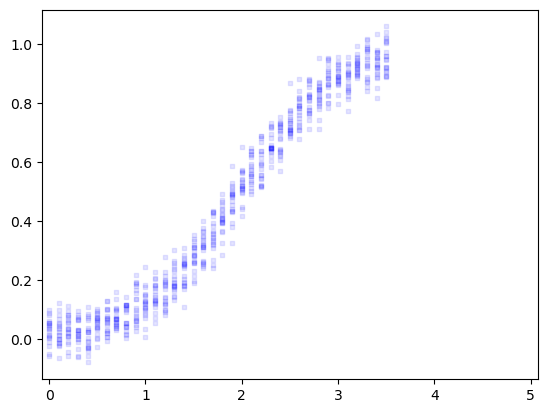
\includegraphics[keepaspectratio]{index_files/figure-latex/notebooks-forster2000_adapted-fig-known-data-output-1.png}}

}

\end{figure}%

\textsubscript{Source:
\href{https://hugetim.github.io/justify-predictive/notebooks/forster2000_adapted-preview.html\#cell-fig-known-data}{Forster
(2000) adapted}}

And suppose your candidate methods for doing so are using Gaussian
polynomial models up to degree 4, with the question being which degree
to use. Although the higher degree models are clearly able to fit the
known values of \(y\) more closely, they are not necessarily better able
to predict the unknown values. For example, here are the 4th degree
polynomial method's predictions:

\begin{figure}[H]

\caption{\label{fig-poly4-predict}POLY-4 Prediction}

\centering{

\pandocbounded{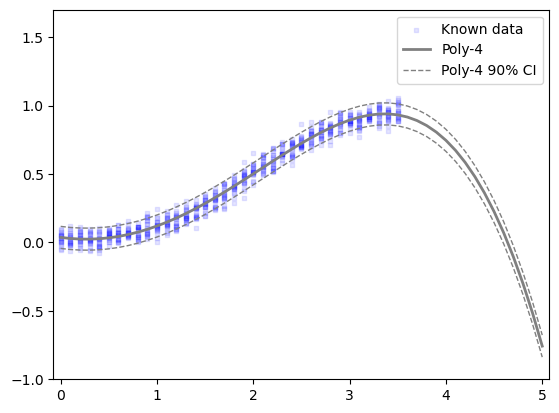
\includegraphics[keepaspectratio]{index_files/figure-latex/notebooks-forster2000_adapted-fig-poly4-predict-output-1.png}}

}

\end{figure}%

\textsubscript{Source:
\href{https://hugetim.github.io/justify-predictive/notebooks/forster2000_adapted-preview.html\#cell-fig-poly4-predict}{Forster
(2000) adapted}}

Those predictions may not look intuitively plausible, but who is to say
that that is not how the pattern would continue? Instead of relying on
intuition, we ought to evaluate how well this and the other methods are
able to make similar predictions for held-out data that we do know. For
simplicity of exposition, consider a prediction class in which the only
known prediction task is to predict \(y\) for \(x\) from 2.6 through
3.5, given the data for \(x\) from 0 to 2.5.\footnote{Similar results
  are obtained using the following tasks as the known prediction class:
  given the data for \(x\) between 0 and 3.4, predict \(y\) for
  \(x=3.5\) (the closest analogy to predicting for \(x=3.6\) given all
  the known data); given the data for \(x\) between 0 and 2.5, predict
  \(y\) for \(x=3.5\) (arguably the closest analogy for predicting \(y\)
  at \(x=5\)); and likewise the eight tasks in between of predicting
  \(y\) for \(x=3.5\) given the data for \(x\) betwen 0 and 2.6, between
  0 and 2.7, and so on; and, finally, given the data for \(x\) between 0
  and 2.4, predict \(y\) for \(x\) between 2.5 and 3.4, inclusive.
  Weighting each of these tasks equally provides a suite of tasks that
  is roughly representative of the tasks of interest: predicting \(y\)
  for each of the \(x\) values 3.6, 3.7, \ldots, 4.9, 5.0. Even this is
  perhaps too small and simple a class. A different suite of tasks, with
  different weights, could just as well be chosen. Ideally, the
  selection of a predictive method will not depend on the choice among
  reasonable such prediction classes. If it does, that tells you
  something about uniqueness, which is discussed further below.} Here is
how the 4th degree method performs on this prediction task:

\begin{figure}[H]

\caption{\label{fig-poly4-eval}POLY-4 Hold-out Evaluation}

\centering{

\pandocbounded{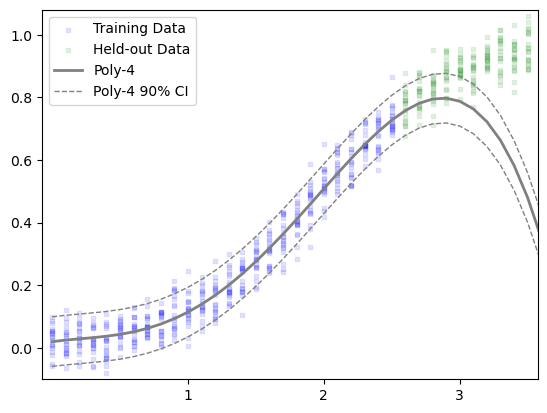
\includegraphics[keepaspectratio]{index_files/figure-latex/notebooks-forster2000_adapted-fig-poly4-eval-output-1.png}}

}

\end{figure}%

\textsubscript{Source:
\href{https://hugetim.github.io/justify-predictive/notebooks/forster2000_adapted-preview.html\#cell-fig-poly4-eval}{Forster
(2000) adapted}}

By contrast, the linear, 1st degree method, which performs best on this
task, looks like this:

\begin{figure}[H]

\caption{\label{fig-poly1-eval}POLY-1 Hold-out Evaluation}

\centering{

\pandocbounded{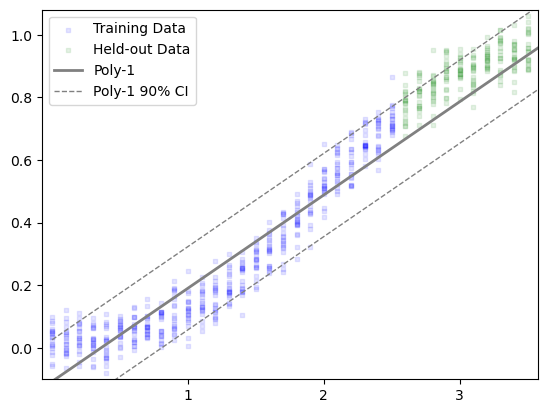
\includegraphics[keepaspectratio]{index_files/figure-latex/notebooks-forster2000_adapted-fig-poly1-eval-output-1.png}}

}

\end{figure}%

\textsubscript{Source:
\href{https://hugetim.github.io/justify-predictive/notebooks/forster2000_adapted-preview.html\#cell-fig-poly1-eval}{Forster
(2000) adapted}}

The linear method performs better both because the central tendency it
predicts is closer to the true data and because it predicts a wider
standard deviation. In other words, the close fit of Poly-4 to the
training data actually hurts its predictive performance by being
``overconfident.''

So, among these candidate methods, Poly-1 is best at the hold-out
predictive task.\footnote{This is a form of ``generalization test,''
  with reference to (Busemeyer and Wang 2000).} And that is why it
should be used for the prediction of interest. It is closest to the
method for reliably predicting the relevant probabilities, if such a
method exists.

In this case, Poly-1 is the clear winner, but what if there were another
method with similar performance? That situation would be analogous to
the deterministic prediction case discussed in Section~\ref{sec-multi}
above. Similar performance is analogous to two deterministic methods
being equally successful, but here that is a fuzzy measure rather than a
binary one.\footnote{One possible measure: if one method's predicted
  probabilities were used to simulate new outcomes for the known
  prediction tasks, how likely is it that the alternative method would
  have been chosen?} Likewise, the question of whether the alternative
method produces equivalent predictions is also fuzzy here, and the right
way to quantify it is not immediately clear. Generally, though, an
analogous principle holds: the justification for using Poly-1
presupposes that there is not a similarly successful alternative with
substantially non-equivalent predictions for the task of interest.

Now, if one thought to try fitting the function
\(a_1 + \tanh (x + a_2)\) to the data, that would perform even better
than Poly-1 for this prediction class, and so \emph{that} should be used
(even if it were not known that such a function was used to simulate
these data, as it was).

But the best predictive method for a given purpose will not necessarily
correspond to the true data-generating process. Suppose the data were
actually generated by a regular zigzag curve of high frequency:
\(f(x) = \left| \left( \frac{2}{\lambda} \cdot x \bmod 2 \right) - 1 \right|\))
Unless we have a very large number of observations, the available data
will not be sufficient to distinguish the zigzag curve from a linear
model with uniformly distributed errors---even if it occurred to us to
try fitting a zigzag curve. And attempting to fit a zigzag to a small
data sample will likely result in worse predictions than the simple
linear model.

Identifying the true data-generating process (given limited data) is not
in itself our goal. Rather, the goal is making predictions as accurate
as possible in the context at hand. In many cases, especially in the
softer sciences, we have no hope of correctly specifying the true model
anyhow. Let's look at an example using real data for which that is the
case.

\begin{itemize}
\tightlist
\item
  Add example with real data (height?)
\item
  Try model averaging? Or just acknowledge it as a possibility,
  something that may or may not improve predictive success.
\item
  Make point that concern about generalization is purely a problem of
  the data available. Our intuition is that fitting to one dataset won't
  generalize, but that is based on ``leakage'': our awareness of
  different data. The thing to do is to train on that extra data as
  well. Once trained on all available data, we have nothing else to go
  on to generalize.
\item
  Maybe use (Myrvold and Harper 2002) orbital period chart example for
  an alternative generalization example
\end{itemize}

\section{Justifying a weighted prediction class}\label{sec-class}

Thus far, the argument has presumed an agreed-upon weighted prediction
class, relative to which predictive success is assessed and with
reference to which the use of a successful predictive method is
justified. But where does this prediction class come from and how can it
be justified, in turn. It is not hard to imagine situations in which a
given prediction of unknown information could be conceived of as part of
multiple alternative prediction classes, with conflicting implications
for which predictive method should be used. It this apparent
incommensurability, then, fatal to the argument as a whole?

No, when in doubt, we can expand the prediction class out to the agent's
whole world, weighting according to importance. The prediction tasks are
to predict (all) future observation, using all past observations as
inputs. More narrow prediction classes can ultimately be evaluated by
how well their selected predictive methods perform in terms of this
universal metric of predictive success.

\begin{itemize}
\tightlist
\item
  Yet how can cross-validation (or, the exchangeability-type assumptions
  involved) be justified?
\end{itemize}

\section{Answering objections to Reichenbach's pragmatic
justification}\label{sec-induct}

This rationale for using successful predictive methods shares some
things in common with Reichenbach's pragmatic vindication of induction.
This section clarifies how the two arguments are related and addresses
the most prominent objections to Reichenbach's argument, as summarized
by (Henderson 2022).

The key commonality is that Reichenbach, while clearly acknowledging
that using induction is not sufficient for success, argued that it is
\emph{necessary}. ``I do not know whether an operation will save the
man, but if there is any remedy, it is an operation.''\footnote{(Reichenbach
  1938 {[}2006: 349{]}), as quoted in (Henderson 2022).}

\begin{itemize}
\tightlist
\item
  Reply to Lange fisherman argument
\end{itemize}

In terms of the principle he was trying to justify, what is sometimes
referred to as ``straight rule'' induction, can be thought of as a
particular form of predictive method: predict the future frequency of a
boolean event to be within a small interval of the observed relative
frequency, \(m/n\).

Reichenbach differed, however, in how he defined success: ``to find
series of events whose frequency of occurrence converges towards a
limit.''\footnote{(Reichenbach 1938 {[}2006: 350{]}), as quoted in
  (Henderson 2022).} Defining success as convergence toward a limit
obstructs Reichenbach from demonstrating that straight-rule induction is
necessary for success. As he acknowledges himself, infinitely many
successful alternative rules can be constructed as the straight-rule
plus some \(c_n\), as long as the \(c_n\) which converges to zero as
\(n\) increases.\footnote{His main attempt to nevertheless salvage a
  unique status for straight-rule induction is to claim that it has the
  ``smallest risk'' of delaying convergence, that it is most likely to
  approximate the limit well for smaller values of \(n\).((Reichenbach
  1938 {[}2006: 355-356{]}), as quoted in (Henderson 2022)) This
  alternative measure of success is more akin to that of
  Section~\ref{sec-prob} above, but Reichenbach did not have the benefit
  of cross-validation being an established concept in the statistics of
  his time.} By contrast, the approach here identifies a unique best
predictive method, based on its currently known predictive track record.

\begin{itemize}
\tightlist
\item
  Add concluding paragraph re short run vs.~long run.
\end{itemize}

\section{Schurz's justification for induction}\label{sec-schurz}

\begin{itemize}
\tightlist
\item
  contrast with more recent pragmatic attempt (ML-inspired formulation
  that doesn't actually fit with ML practice), addressing its critique
  of simply adopting the ``most successful'' predictive method
\end{itemize}

\section{Probability}\label{sec-intprob}

As Wesley Salmon put it, the challenge of providing an adequate
philosophical interpretation of probability is ``Hume's problem of
induction all over again in slightly different terminology.''\footnote{(Salmon
  2017) (p.~65)} So, while this is not the place for an in-depth
treatment of the philosophy of probability, it is worth briefly noting
that the concept of ``best predictive method'' described above also
provides an interpretation of probability.

According to Salmon, the fundamental challenge in interpreting
probability is ``to satisfy simultaneously the criteria of
ascertainability and applicability.''\footnote{Ibid.} Ascertainability
means it is possible to determine what the value of a particular
probability is, at least in principle, whereas applicability means that
a probability should have practical significance. In brief,
ascertainability is the primary challenge for the frequency
interpretation of probability, whereas more subjective conceptions of
probability as degree of belief tend to fall short on applicability. The
predictive method approach advocated here, defining probability as the
predicted probability for a given event, straightforwardly meets the
criteria of applicability, and it also provides a new angle on
ascertainability. The probability distribution in a given predictive
context is that indicated by the predictive method with the greatest
predictive success, the highest average log-likelihood for the cases in
a predictive class. In principle, it may be defined as the probability
distribution of the true best predictive method, that which would be
most successful for as-yet unobserved instances as well as those already
known. In practice, it may be ascertained according to the best known
predictive method.

The predictive approach improves upon the frequency interpretation in
its handling of the single case, unrepeated or unrepeatable
events.\footnote{See (Hájek 2023) for further discussion.} \ldots{}

\section{Conclusion}\label{sec-conclude}

In his book \emph{The Knowledge Machine}, Michael Strevens provides a
compelling account of how science works, a lucid synthesis of decades of
insights from history and philosophy of science, albeit with one
unsettling limitation. Strevens makes the quandaries of philosophers
actually fun to read about, including David Hume's problem of induction,
the lack of a reasoned justification for generalizing from experience.
On the stakes of this problem, he quotes Bertrand Russell, who said that
if inductive reasoning cannot be justified, ``there is no intellectual
difference between sanity and insanity'' (p.~17) And Russell is not
alone. As Strevens puts it, almost all philosophers of science ``believe
that induction is essential to human existence'' (p.~21).\footnote{``Some
  believe that Hume's problem must have a solution---that is, a
  philosophical argument showing that it is reasonable to suppose that
  nature is uniform in certain respects\ldots{} Some believe, like Hume
  himself, that it has no solution but that we must go on thinking
  inductively regardless, both in our science and in our everyday
  lives'' (p.~21). Strevens does not make clear to which camp he himself
  belongs.} Yet, ``there is still no widely accepted justification for
induction'' (p.~17).

Any inductive inference from known information to unknown can be thought
of as a prediction, broadly construed, so the argument above amounts to
a pragmatic justification for induction. Aside from providing a
foundational rationale for our common-sense attitudes, something that
perhaps only philosophers care about, this refined grounding for
inductive reasoning has practical implications for how science should be
conducted and interpreted. But such implications are for future work.
For now I would just situate the relevance of these philosophical
considerations in the context of Strevens' account of science in
\emph{The Knowledge Machine.}

Strevens' book goes on to argue that the power of modern science stems
from how it directs scientists to relentlessly prioritize tedious
empirical observations over the aesthetic, religious, or philosophical
considerations to which pre-modern students of the natural world
dedicated the bulk of their attention and writing. But Strevens never
returns to the basic question of how generalizing from all those
meticulous observations can be justified in the first place.\footnote{Strevens
  gestures toward ``Baconian convergence'' but does not attempt to
  explain why this seems to work so well rather than being defeated by
  the underdetermination that seems so inevitable when confirmation
  theory is considered in the abstract.} It almost seems as if Strevens
hopes his readers, despite his forceful presentation of Hume's problem
of induction in the first chapter, will have safely forgotten this
disturbing quandary by the end of the subsequent thirteen chapters. The
justification of inductive reasoning presented here aims to provide a
more satisfying account for why all that careful observation Strevens
celebrates matters: by eliminating rival predictive methods, we are left
not with a bewildering infinitude of theories yet capable of fitting our
still-finite observations but rather, for so many practical purposes, a
single relevant predictive method, enabling our ever-expanding technical
mastery.

\section*{References}\label{references}
\addcontentsline{toc}{section}{References}

\phantomsection\label{refs}
\begin{CSLReferences}{1}{0}
\bibitem[\citeproctext]{ref-barnes2022}
Barnes, Eric Christian. 2022. {``Prediction Versus Accommodation.''} In,
edited by Edward N. Zalta and Uri Nodelman, Winter 2022. Metaphysics
Research Lab, Stanford University.
\url{https://plato.stanford.edu/archives/win2022/entries/prediction-accommodation/}.

\bibitem[\citeproctext]{ref-busemeyer2000}
Busemeyer, Jerome R, and Yi-Min Wang. 2000. {``Model Comparisons and
Model Selections Based on Generalization Criterion Methodology.''}
\emph{Journal of Mathematical Psychology} 44 (1): 171--89.
\url{https://doi.org/10.1006/jmps.1999.1282}.

\bibitem[\citeproctext]{ref-donoho2017}
Donoho, David. 2017. {``50 Years of Data Science.''} \emph{Journal of
Computational and Graphical Statistics} 26 (4): 745--66.
\url{https://doi.org/10.1080/10618600.2017.1384734}.

\bibitem[\citeproctext]{ref-forster2008}
Forster, Malcolm. 2008. {``Prediction.''} In, 433441. Routledge.
\url{https://www.taylorfrancis.com/chapters/edit/10.4324/9780203000502-47/prediction-malcolm-forster}.

\bibitem[\citeproctext]{ref-forster2000}
Forster, Malcolm R. 2000. {``Key Concepts in Model Selection:
Performance and Generalizability.''} \emph{Journal of Mathematical
Psychology} 44 (1): 205231.
\url{https://www.sciencedirect.com/science/article/pii/S0022249699912841}.

\bibitem[\citeproctext]{ref-forster1994}
Forster, Malcolm, and Elliott Sober. 1994. {``How to Tell When Simpler,
More Unified, or Less Ad Hoc Theories Will Provide More Accurate
Predictions.''} \emph{The British Journal for the Philosophy of Science}
45 (1): 1--35. \url{http://www.jstor.org/stable/687960}.

\bibitem[\citeproctext]{ref-huxe1jek2023}
Hájek, Alan. 2023. {``Interpretations of Probability.''} In, edited by
Edward N. Zalta and Uri Nodelman, Winter 2023. Metaphysics Research Lab,
Stanford University.
\url{https://plato.stanford.edu/archives/win2023/entries/probability-interpret/}.

\bibitem[\citeproctext]{ref-henderson2022}
Henderson, Leah. 2022. {``The Problem of Induction.''} In, edited by
Edward N. Zalta and Uri Nodelman, Winter 2022. Metaphysics Research Lab,
Stanford University.
\url{https://plato.stanford.edu/archives/win2022/entries/induction-problem/}.

\bibitem[\citeproctext]{ref-kaufman2012}
Kaufman, Shachar, Saharon Rosset, Claudia Perlich, and Ori Stitelman.
2012. {``Leakage in Data Mining: Formulation, Detection, and
Avoidance.''} \emph{ACM Transactions on Knowledge Discovery from Data} 6
(4): 1--21. \url{https://doi.org/10.1145/2382577.2382579}.

\bibitem[\citeproctext]{ref-myrvold2002}
Myrvold, Wayne C., and William L. Harper. 2002. {``Model Selection,
Simplicity, and Scientific Inference.''} \emph{Philosophy of Science} 69
(S3): S135--49. \url{https://doi.org/10.1086/341841}.

\bibitem[\citeproctext]{ref-romeijn2022}
Romeijn, Jan-Willem. 2022. {``Philosophy of Statistics.''} In, edited by
Edward N. Zalta and Uri Nodelman, Fall 2022. Metaphysics Research Lab,
Stanford University.
\url{https://plato.stanford.edu/archives/fall2022/entries/statistics/}.

\bibitem[\citeproctext]{ref-salmon1981}
Salmon, Wesley C. 1981. {``Rational Prediction.''} \emph{The British
Journal for the Philosophy of Science} 32 (2): 115--25.
\url{https://doi.org/10.1093/bjps/32.2.115}.

\bibitem[\citeproctext]{ref-salmon2017}
---------. 2017. \emph{The Foundations of Scientific Inference: 50th
Anniversary Edition}. University of Pittsburgh Press.
\url{https://www.jstor.org/stable/j.ctt1s475s3}.

\end{CSLReferences}




\end{document}
